
\section{Dataset}


\begin{figure*}[t]
    \centering
    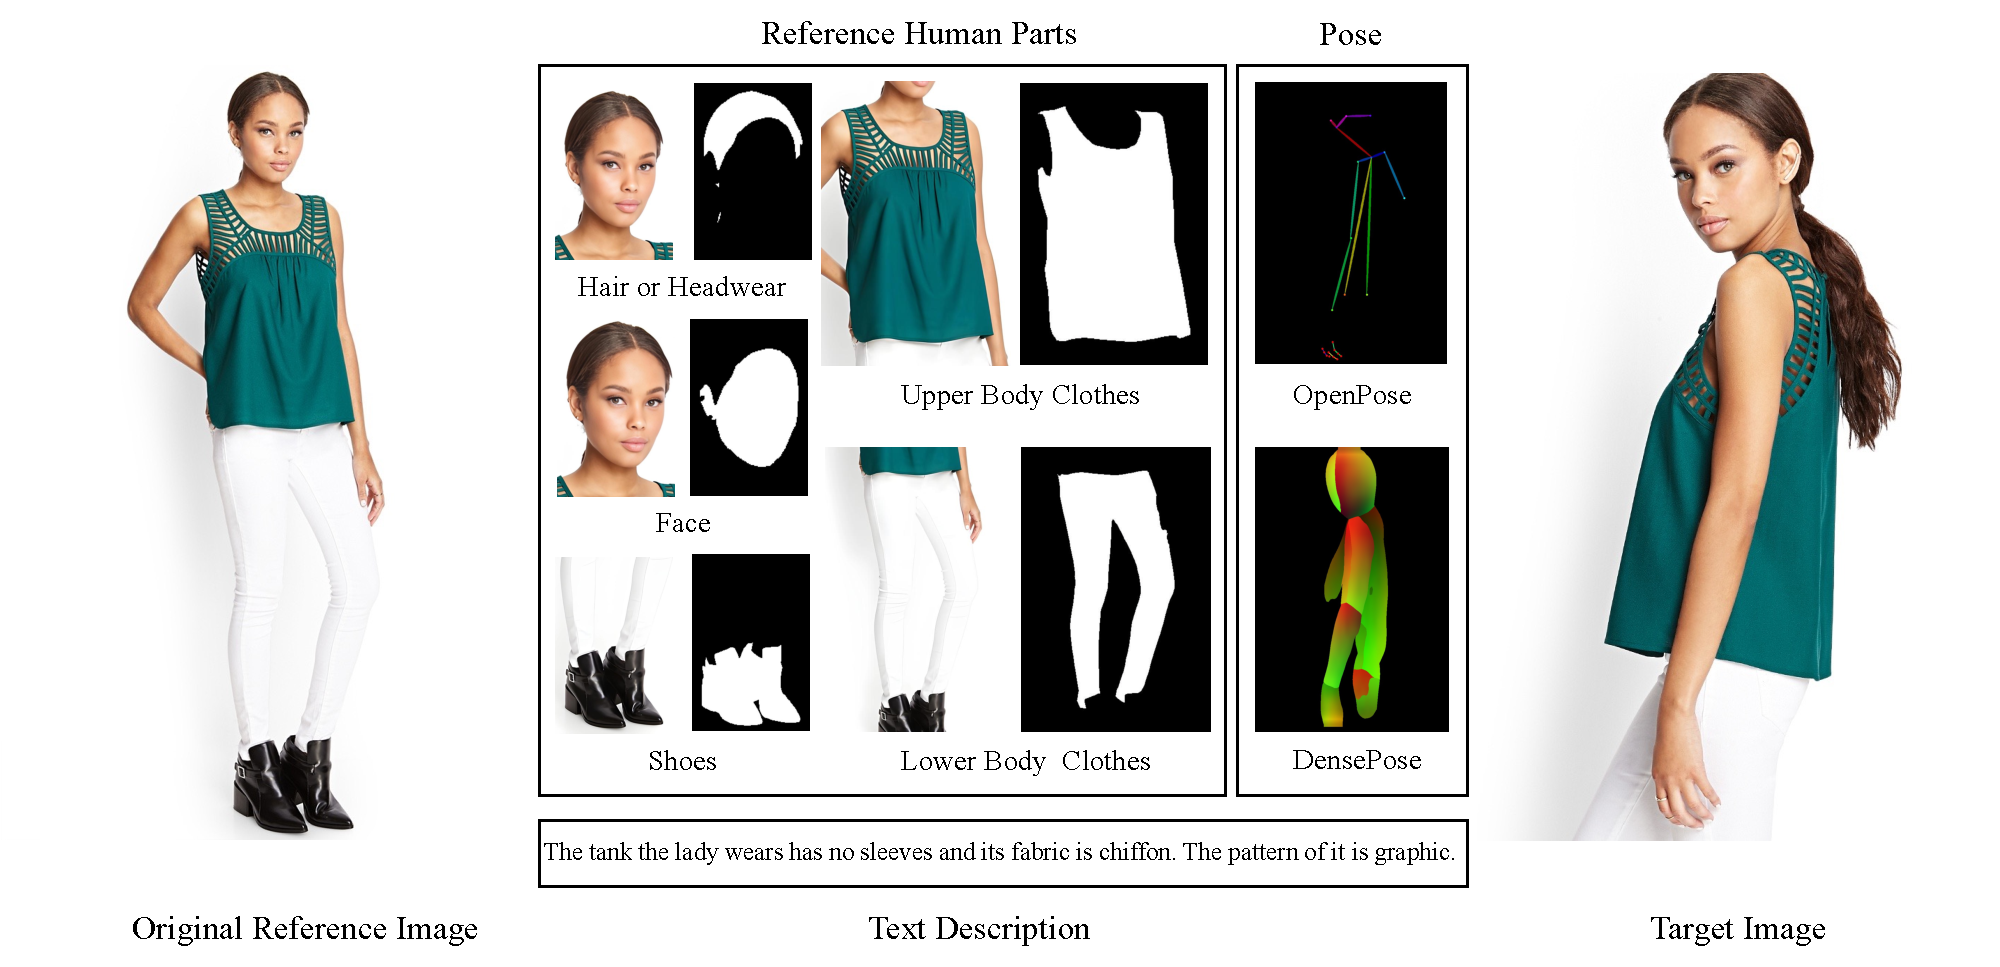
\includegraphics[width=0.95\textwidth]{figure/supp_data_sample.pdf}
    \caption{A sample of reference-target image pair in our dataset. Reference Human Part images are obtained from the reference image based on the human parsing image, while the pose and text description are descriptions of the target image.}
    \label{fig:sample_data}
\end{figure*}

\begin{figure*}[ht!]
    \centering
    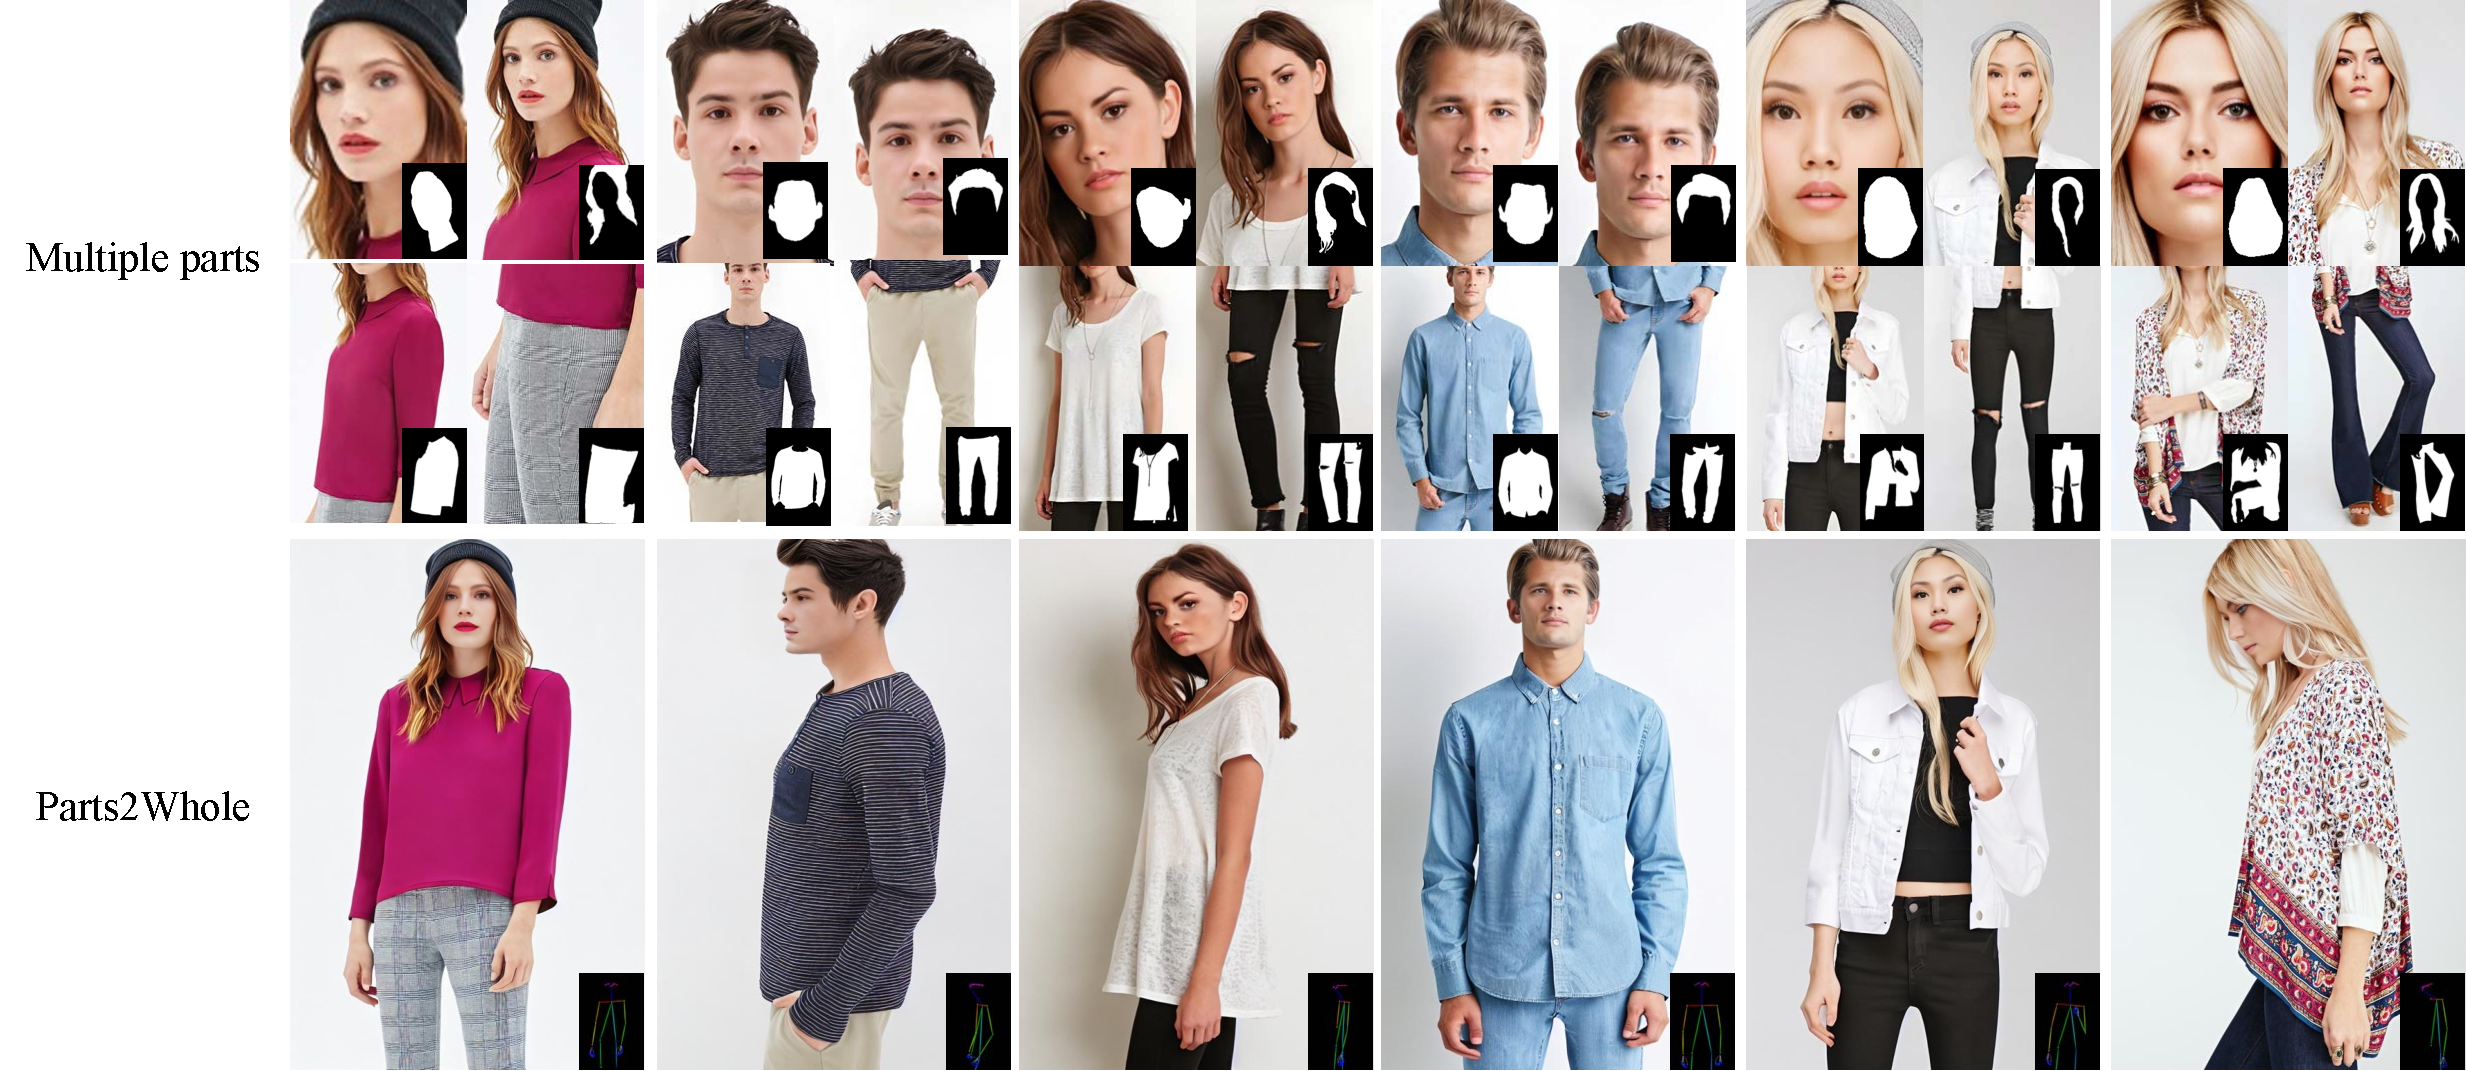
\includegraphics[width=\textwidth]{figure/supp_openpose.pdf}
    \caption{Generated human images with OpenPose as pose condition by Parts2Whole. The upper row displays multiple reference human parts, while the lower row shows the results generated by our Parts2Whole method under the control of reference images and OpenPose image.}
    \label{fig:supp_openpose}
\end{figure*}

Generating the human body from multiple conditional parts is a significant undertaking, but lacking a directly available dataset. The datasets related to this task, such as those for Virtual Try-on\cite{choi2021viton,morelli2022dress,zablotskaia2019dwnet}, primarily suffer from a lack of multiple controllable conditions and are often limited to single control conditions (clothing). Issues with these datasets include a limited variety of clothing types, absence of facial data, low resolution, and lack of textual captions. The DeepFashion-MultiModal dataset~\cite{jiang2022text2human,liuLQWTcvpr16DeepFashion} aligns more closely with our task as it includes a vast array of human body images, the same person and same clothes in different poses, and precise human parsing labels. However, this dataset cannot be used directly and requires data cleansing and further post-processing.

\cparagraph{ID Cleansing.}
In the DeepFashion-MultiModal dataset, there is some confusion with IDs where images of different individuals are mistakenly labeled under the same ID. We start by cleansing these IDs, extracting facial ID features from images tagged with the same ID using InsightFace\cite{deng2018arcface, InsightFaceProject}. Cosine similarity is then used to evaluate the similarity between image ID feature pairs, allowing us to reclassify IDs within the same ID group. After cleansing, images from the same ID and the same clothes are selected if there are two or more images available.

\cparagraph{Building Reference-Target Pair.}
We use images with human parsing labels from the dataset as reference images. Target images are then selected from the same ID and clothing, creating pairs with the reference image.

\cparagraph{Obtaining Reference Human Part.}
We crop the images according to the provided human parsing labels. Specifically, we divide the human image into six parts: upper body clothes, lower body clothes, whole body clothes, hair or headwear, face, and footwear. Each part is cropped according to the human parsing labels to obtain the crop image and corresponding mask image. Due to the low resolution of the cropped parts, we apply Real-ESRGAN\cite{wang2021realesrgan} to enhance the image resolution, thus obtaining clearer reference images.

\cparagraph{Obtaining Target Description.}
Based on the reference human parts, we need to generate images that resemble the target image, requiring a description of the target image. The description is divided into two parts: one for the human body's pose and another for the target image's textual description. For pose information, we utilize DWPose\cite{yang2023dwpose} to generate pose images corresponding to each image, and for DensePose, we use the provided DensePose files from the dataset. The textual description for each image is taken directly from the dataset's accompanying text description.

\cparagraph{Introduction to the Final Dataset.}
Finally, we have constructed a multimodal dataset with approximately 41,500 reference-target pairs derived from the open-source DeepFashion-MultiModal dataset~\cite{jiang2022text2human,liuLQWTcvpr16DeepFashion}. The controllable conditions for each pair are categorized into two main types. The first type is the appearance reference image, which is subdivided into six parts: upper body clothes, lower body clothes, whole body clothes, hair or headwear, face, and footwear. Each image is accompanied by a corresponding mask and has undergone super-resolution processing. These data elements are sourced from the original reference image. The second type is the target description, primarily consisting of pose and text description. The pose is further divided into OpenPose and DensePose, all of which are derived from the target image. A sample of reference-target image pair in our dataset is shown in Fig.~\ref{fig:sample_data}.


